\begin{figure}[htbp]

\begin{center}
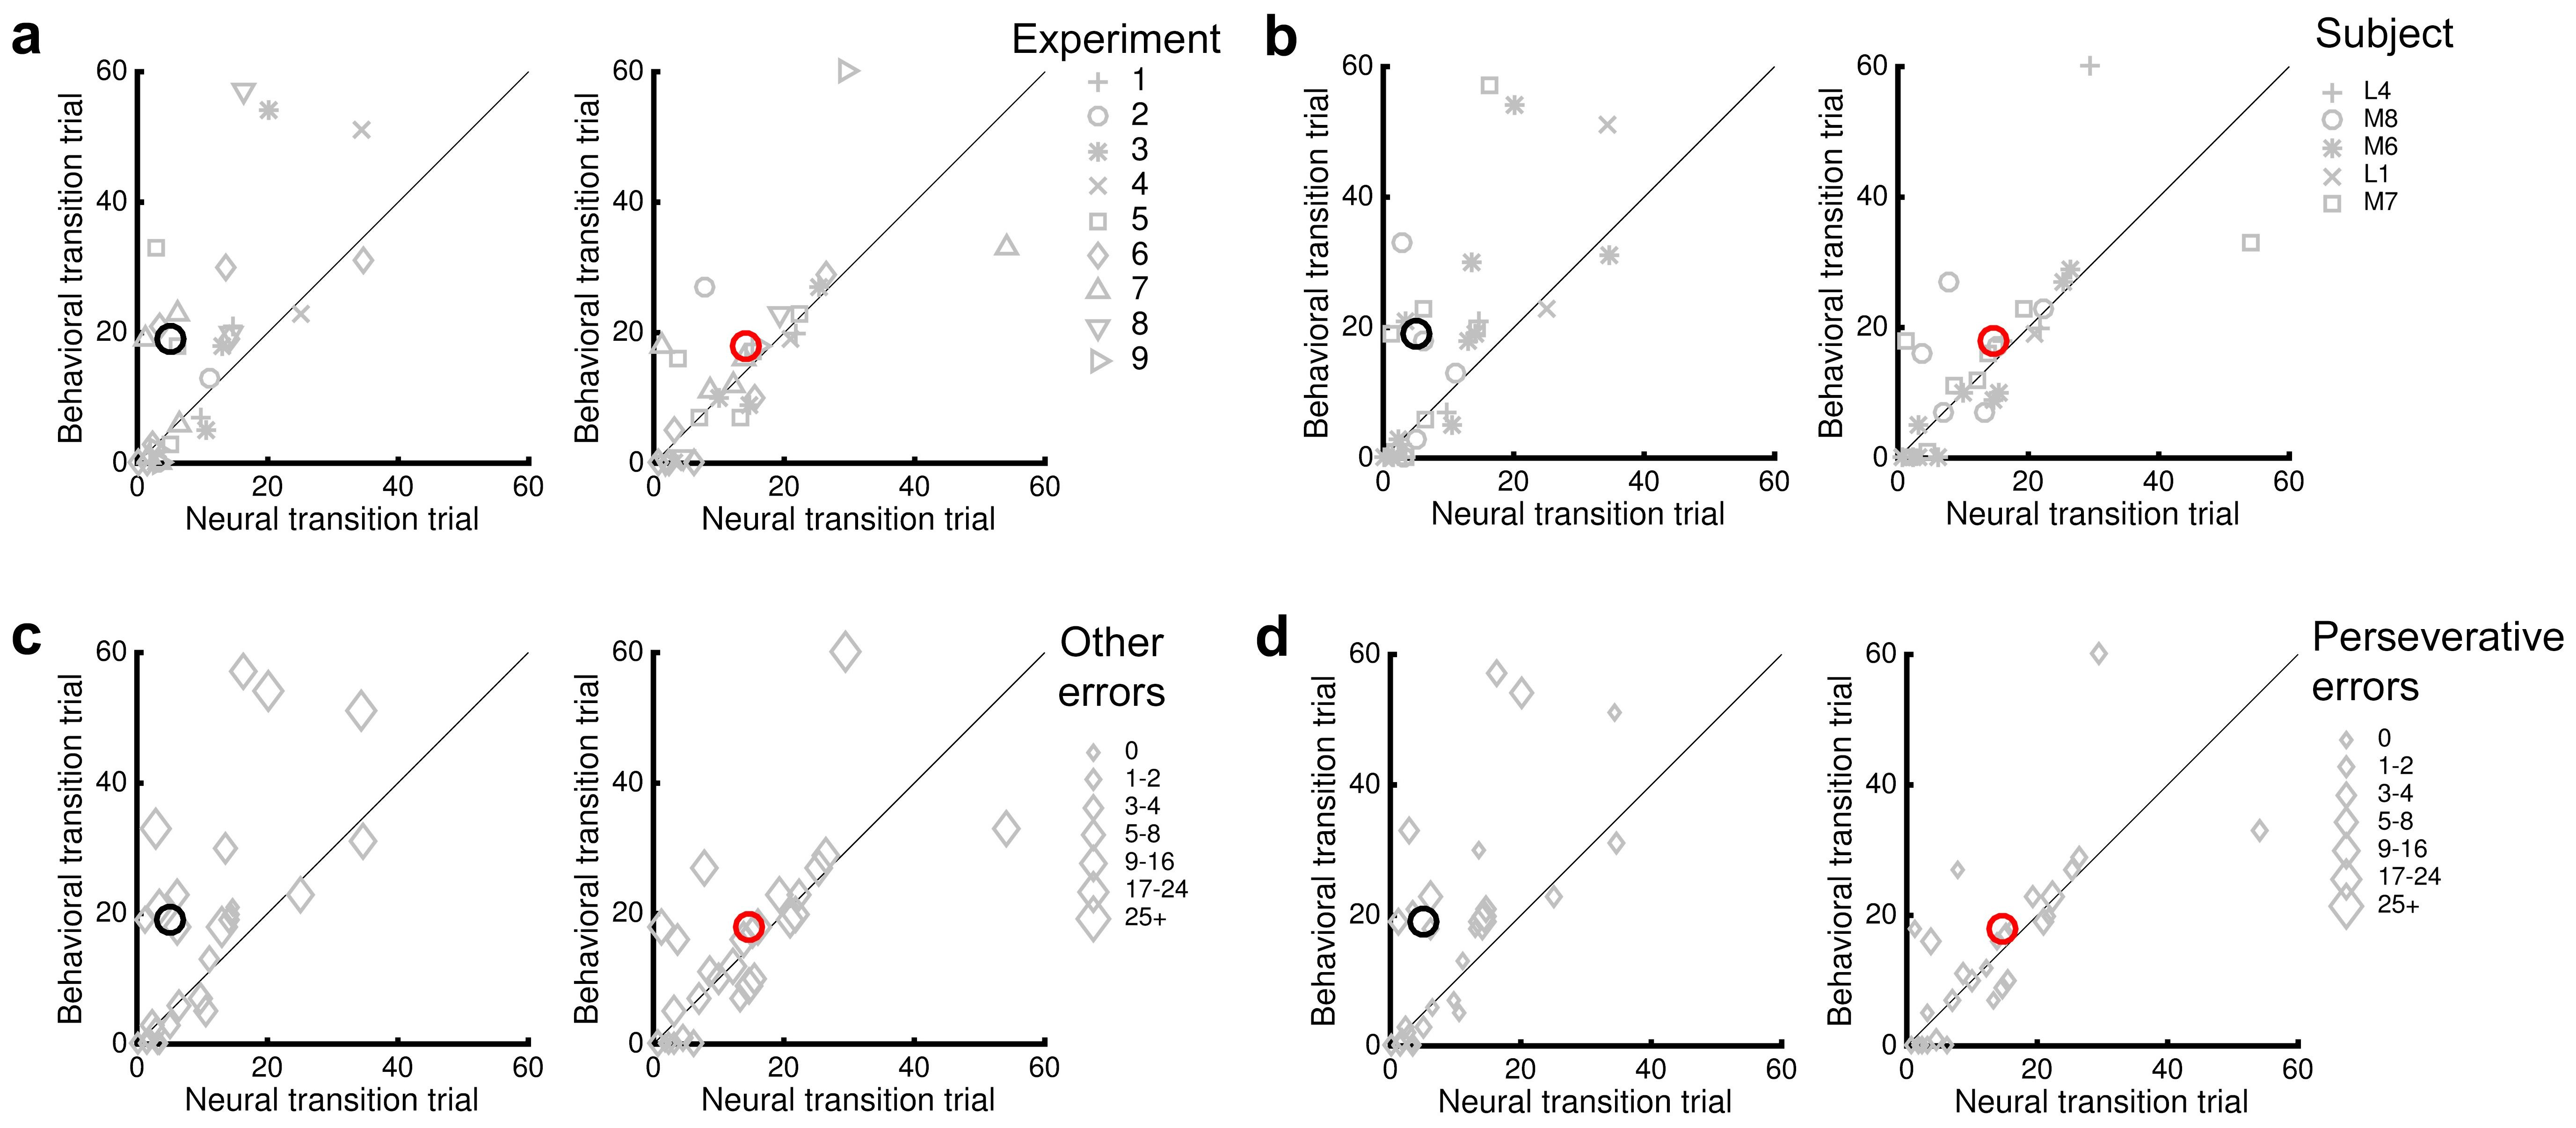
\includegraphics[width=\textwidth]{Figures/Chapter3/NN_figS6.jpg} 
\end{center}

\caption[Relationship between session parameters and neural/behavioral transitions]
{
Relationship between session parameters and neural/behavioral transitions.
(a) Ensemble transition trials plotted against the behavioral transition trial from the same block (see Methods). Each point represents one block switch. Bold circle, median value. Left panel: $n=33$ switches to a sound block from 9 sessions from 5 mice. Right panel: $n=35$ switches to a spatial block from 9 sessions from 5 mice. Symbols denote the different experimental sessions. (b) Same as \emph{a}, except symbols denote the experimental subjects. (c) Same as \emph{a}, except symbol sizes denote the number of other errors in the block. (d) Same as \emph{a}, except symbol sizes denote the number of perseverative errors in the block.
}

\label{fig:NN_figS6}
\end{figure}